Problem regresji liniowej za pomocą spadku gradientowego został poprawnie rozwiązany. Wszystkie kroki zostały przeprowadzone pomyślnie oraz otrzymany prostą opisującą próbki tak, aby dzięki niej mozna było przewidzieć kolejne wartości:
\newline
\large
$$
h(x) = 10473 + 6282.5 * x
$$
\normalsize
\noindent
\newline
Pewność tego wyniku potwierdza utknięcie $J(\theta)$ w globalnym minimum. Jednocześnie uzyskany wykres już bez dokładnego przyglądania się obrazuje to, że uzyskana prosta jak najbardziej opisuje te próbki i przewidzi z małym błędem dodane w przyszłości.


	\begin{figure}[H]
    \centering
    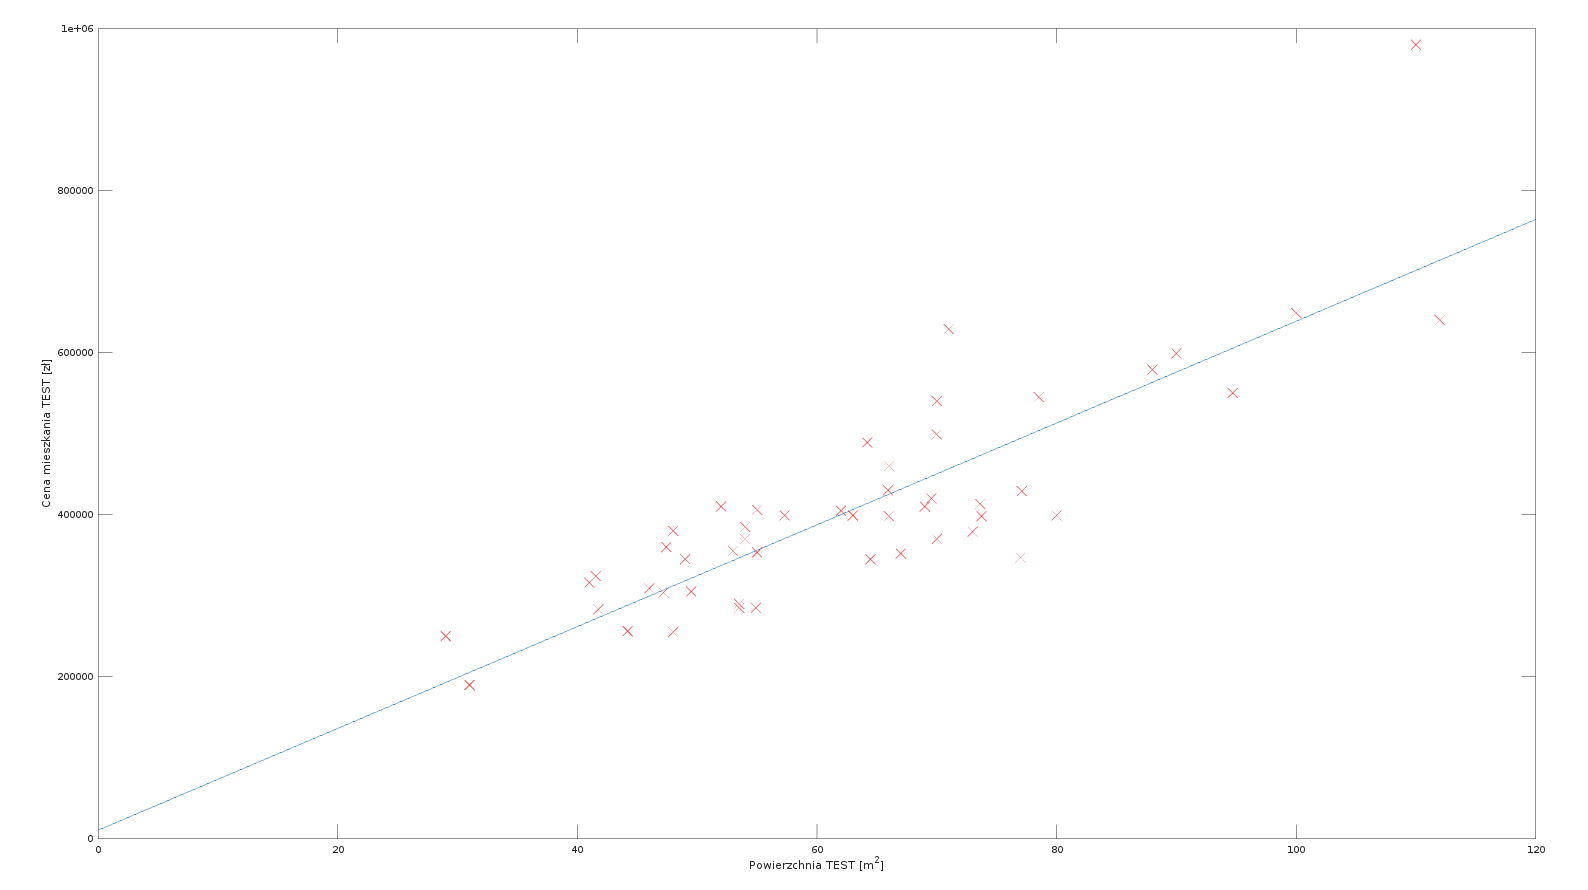
\includegraphics[scale=0.22]{PNG/perfect_grad.png}
    \caption{Idealna regresje znaleziona przez spadek gradientowy}
    \label{lamana}
	\end{figure}
	

Na sam koniec podsumowujmy, dlaczego spaek gradientowy jest jedną z lepszych metod znajdywania predykcji. Po pierwsze możemy posiadać nieskończoną ilość danych wejściowych - nie tylko ze względu na ilość, ale też ich rodzaj (np. metraż, odległość od centrum). Po drugie jesteśmy w stanie łatwo sprawdzić czy nasz algorytm zadziałał poprawnie. Jesteśmy również w stanie w łatwy sposób przeprowadzić badania na nowych próbkach, ponieważ posiadamy rzeczywiste odwzorowanie i nie musimy uruchamiać algorytmu przy każdej nowej próbce, a wystarczy użyć uzyskanego wzoru.